\section{Versuchsanordnung und -durchführung}

\subsection{Versuchsaufbau und Elektronik} \label{AufbauElektronik}

Der Aufbau dieses Versuchs ist in Abbildung \ref{Aufbau} schematisch dargestellt und besteht aus einer Vakuumkammer, zwei Detektoren, drei Mylar-Folien, einer Strahlungsquelle, der signalverarbeitenden Elektronik sowie einem Computer.
\noindent Die Strahlungsquelle ist Americium-$241$, welches nahezu ausschließlich unter Emission von $\alpha$-Strahlung in angeregte Kernzustände von Neptunium-$237$ zerfällt.
Im Innern der Vakuumkammer ist die Strahlungsquelle auf einen Folienhalter gerichtet, in welchem drei unterschiedlich dicke Mylar-Folien eingesetzt sind.
Durch die Drehung der Folien lässt sich deren effektive Dicke verändern, sodass die Energie der hindurchgehenden $\alpha$-Teilchen variiert wird und kontinuierliche $\alpha$-Energien entstehen.
Hinter dem Folienhalter sind nacheinander die zwei Detektoren positioniert.
Bei den beiden Halbleiterdetektoren handelt es sich um Si-Oberflächensperrschicht-Detektoren.
Dabei ist der von einem einfallenden $\alpha$-Teilchen zuerst getroffene Detektor ungefähr \SI{7}{\micro\meter} dick und wird als $\Delta E$-Detektor bezeichnet.
Der dem $\Delta E$-Detektor nachstehende sogenannte $E$-Detektor ist circa \SI{200}{\micro\meter} dick.
An den $\Delta E$-Detektor wird eine Spannung von \SI{3}{\volt} und an den $E$-Detektor eine Hochspannung von \SI{250}{\volt} angelegt.
Die Folien und der $\Delta E$-Detektor sind aus dem $\alpha$-Strahlengang entfernbar.
Beide Detektoren sind jeweils an Vorverstärker mit der Modellbezeichnung "Canberra 970" angeschlossen, welche über externe Spannungsquellen versorgt werden.
Die zwei Vorverstärker sind jeweils mit einem Hauptverstärker verbunden.
Wobei einer dieser beiden Hauptverstärker vom Typ "Canberra 2022" und der andere vom Typ "Ortec 575" ist.
Die von den zwei Hauptverstärkern ausgehenden unipolaren Signale werden von einem CAMAC ADC (engl. \emph{analog-to-digital converter}) mit der Modellbezeichnung "LeCroy 2259B" ausgelesen.
Der CAMAC ADC ist über eine CAMAC-Karte mit dem Computer verbunden, welcher über eine entsprechende Datenaufnahme-Software verfügt.
Zusätzlich wird das Signal des dem $E$-Detektor zuzuordnenden Vorverstärkers an einen Diskriminator vom Typ "Ortec 584" weitergeleitet.
Dieser gibt das Signal erst ab einer bestimmten Signalhöhe weiter, sodass das Hintergrundrauschen herausgefiltert wird.
\begin{figure}[H]
	\centering
	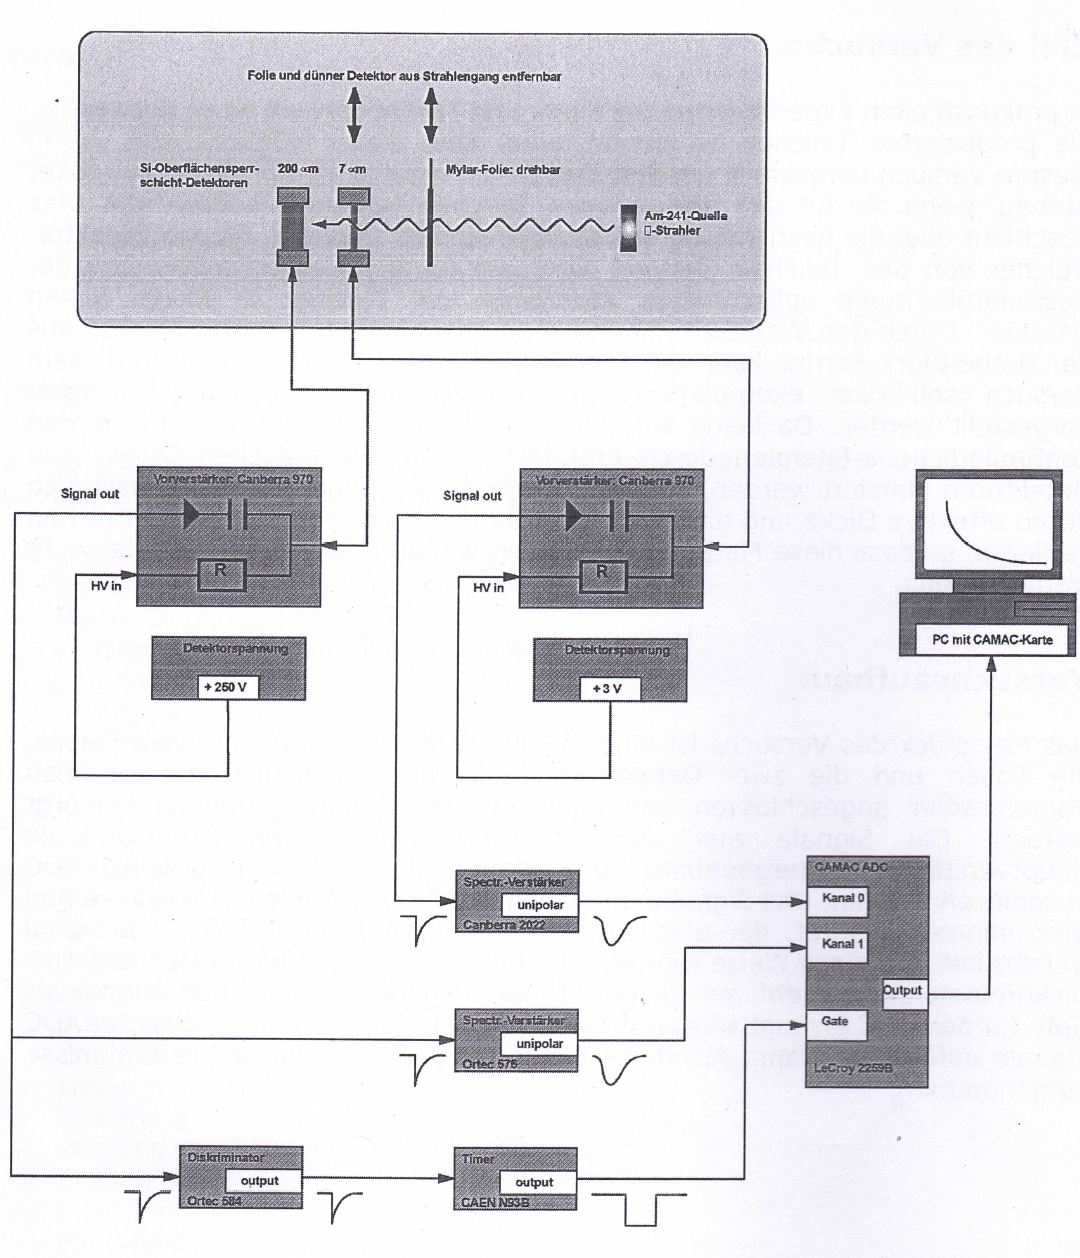
\includegraphics[width=\textwidth]{img/Aufbau}
	\caption{In dieser Abbildung ist der schematische Aufbau dieses Versuchs in Form eines Blockschaltbilds dargestellt. Die Abbildung wurde der Versuchsanleitung\cite{wwu} entnommen und anschließend bearbeitet.}
	\label{Aufbau}
\end{figure}
Der Diskriminator ist an einen Timer mit der Modellbezeichnung "CAEN N93B" angeschlossen, welcher das Eingangssignal in ein Rechtecksignal umwandelt.
Letzteres dient als Gate für den nachstehenden CAMAC ADC und gibt den Zeitraum an, bei dem dieser Signale aufnehmen kann.
Auf diese Weise werden nur koinzidente Ereignisse aufgenommen.

\subsection{Durchführung}

Zunächst wird der $E$-Detektor kalibriert.
Dazu wird der $\Delta E$-Detektor und der Folienhalter samt Mylar-Folien aus dem $\alpha$-Strahlengang entfernt.
Anschließend soll das vom $E$-Detektor gemessene $\alpha$-Energiespektrum von $^{241}$Am aufgenommen werden.
Diese Kalibrierungsmessung wird solange durchgeführt, bis eine adäquate Anzahl von Ereignissen registriert worden ist.

Im zweiten Teilexperiment soll die Kalibrierung und die Dickebestimmung des $\Delta E$-Detektors stattfinden.
Dafür wird der $\Delta E$-Detektor wieder in den $\alpha$-Strahlengang eingesetzt.
Danach werden die von beiden Detektoren gemessenen $\alpha$-Energiespektren mit einer adäquaten Anzahl von Ereignissen aufgenommen.

Nun soll mit Hilfe des $E$-Detektors die Dicke von einer, zwei und drei Mylar-Folien bestimmt werden.
Im Zuge dessen wird der $\Delta E$-Detektor erneut aus dem $\alpha$-Strahlengang entfernt und zuerst der Folienhalter mit einer Mylar-Folie eingesetzt, sodass sich die Folie zwischen der Strahlungsquelle und dem $E$-Detektor befindet.
Dabei ist die Längsseite der Folie senkrecht zum $\alpha$-Strahlengang auszurichten, was einem Winkel von \SI{0}{\degree} entspricht.
Anschließend wird das vom $E$-Detektor gemessene $\alpha$-Energiespektrum aufgenommen.
Diese Messung soll mit zwei und mit drei Folien wiederholt werden.

Im letzten Teilexperiment wird der Energieverlust im $\Delta E$-Detektor bei verschiedenen $\alpha$-Energien bestimmt.
Dazu wird der $\Delta E$-Detektor wieder in den $\alpha$-Strahlengang eingesetzt.
Unter Verwendung des CAMAC-Messsystems sollen nun koinzidente Ereignisse gemessen werden.
Dies bedeutet, dass nur dann ein Messwert aufgenommen wird, wenn in beiden Detektoren zur gleichen Zeit ein Ereignis stattfindet.
Hierbei ist anzumerken, dass die von den Detektoren ausgehenden Signale nicht wirklich koinzident sind.
Aufgrund der hohen Geschwindigkeit eines einfallenden $\alpha$-Teilchens und des geringen Abstands zwischen dem $\Delta E$-Detektor und dem $E$-Detektor entsteht jedoch eine scheinbare Koinzidenz.
Zunächst wird der Folienhalter samt Mylar-Folien aus dem $\alpha$-Strahlengang entfernt und das Energiespektrum mit Hilfe beider Detektoren aufgenommen.
Für jede der drei Mylar-Folien wird der Folienhalter mit der entsprechenden Folie in den $\alpha$-Strahlengang gebracht und der Winkel zwischen der Längsseite einer Folie und dem $\alpha$-Strahlengang in \SI{15}{\degree}-Schritten von \SIrange{0}{60}{\degree} variiert.
Bei jedem dieser \SI{15}{\degree}-Schritte wird unter Verwendung beider Detektoren das Energiespektrum mit einer adäquaten Anzahl von Ereignissen aufgenommen.
Anzumerken ist, dass vor allem bei niedrigen Zählraten die Messzeit ausreichend groß gewählt werden sollte, um genügend Datenpunkte sammeln zu können.
